\section{Planificación General}

\subsection{Introducción}
\quad En esta sección se describe la planificación temporal del proyecto, así como el beneficio monetario que se espera de la aplicación.\\

\subsection{Planificación}

\quad El desarrollo de este proyecto se inició seriamente en Marzo de 2019, pero debido a asuntos personales del autor, no se pudo dedicar todo el tiempo necesario desde el mismo inicio, lo que provocó que la implementación y pruebas se retrasaran en el marco temporal.\\

\quad La planificación temporal de este proyecto se divide en una serie de etapas bien diferenciadas, mostradas en el siguiente diagrama de Gantt:\\

\begin{figure}[htb]
	\centering
	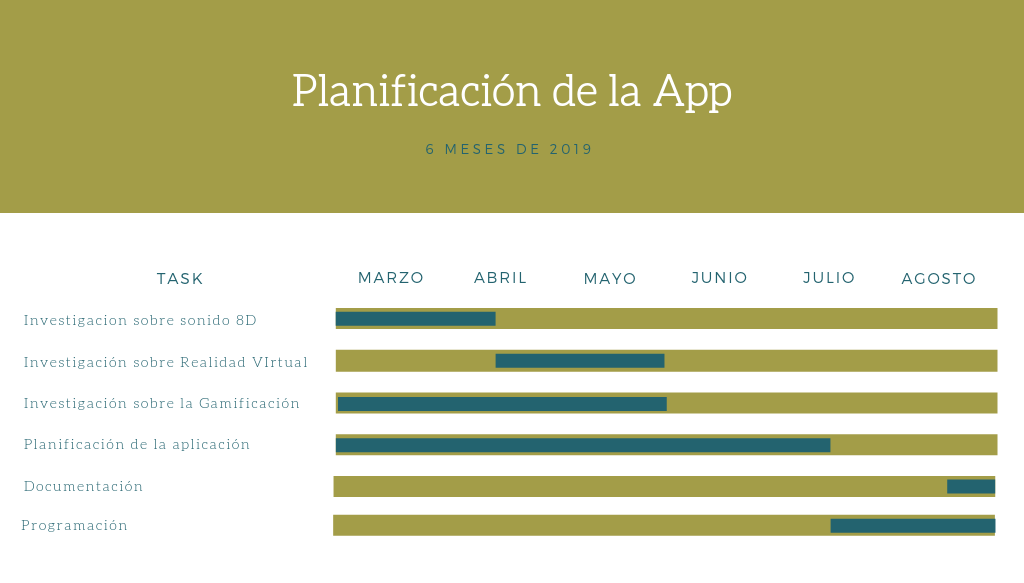
\includegraphics[width=1.2\textwidth]{./imagenes/diagramaGantt}
	\caption{Distribución del tiempo de desarrollo de la aplicación}
\end{figure}

\subsection{Tareas}

\quad Ahora pasamos a repasar las distintas tareas que podemos encontrar a lo largo de todo el periodo de desarrollo, Para facilitar la comprensión las agrupamos según las diferentes etapas del desarrollo.\\

\subsubsection{Etapa de análisis}

\quad Durante esta etapa se tuvo que analizar tanto las herramientas como los  diferentes planteamientos para afrontar el problema al que nos enfrentamos. En concreto, gran parte del tiempo se dedicó a comprender tanto el algoritmo 8D como las diferentes implementaciones de la realidad virtual.\\

\quad Hay que tener en cuenta también que es importante  conocer cómo funciona tanto el 8D como la realidad virtual, pero los conceptos no se quedan solo ahí, ya que una parte fundamental es la inmersión dentro de la aplicación y cómo emplearla de forma natural.\\

\quad Esto provocó un estudio exhaustivo de las diferentes formas de implementar un interfaz de usuario en realidad virtual, así como las mejores maneras de interactuar con ellas.\\

\quad Quizás el análisis que más tiempo llevó fue el del algoritmo 8D, pues requería entender desde cero un concepto nuevo para mi, ya que al principio lo entendía de una manera totalmente errónea. A poriori, este debe de trabajar desde la ubicación del usuario al foco, pero los cálculos y las implementaciones vistas me han demostrado que se hace un enfoque bidireccional, de forma que se pueda calcular el volumen del sonido de una forma más precisa.\\

\quad También cabe destacar que desde el principio planteé la aplicación a dispositivos móviles, ya que cualquier otra opción implicaría inevitablemente una inversión de dinero que no podía asumir.\\

\subsubsection{Etapa de diseño} 

\quad Abordados ya los conceptos que debía tener claros, empecé con el planteamiento de la aplicación.\\

\quad La primera idea fue hacer un entorno en un bosque donde escuchar el sonido de varios pájaros revoloteando, y de hecho este planteamiento es que lleva a la escena tres de la aplicación, pero me di cuenta que entonces dejaría muchos conceptos sin explorar, como el eco en una habitación o interactuar con un sujeto que se dirija a ti específicamente.

\quad Este planteamiento fue el que me llevó a buscar nuevas ideas para las escenas, dando lugar a las escenas uno y dos, donde tendremos que buscar a un objetivo invisible y experimentar con un emisor de sonido en un entorno con eco respectivamente.\\

\quad Parte de esta etapa la dediqué también a buscar diferentes assest que pudieran servir para completar los entornos en lo que se moverá el usuario, haciendo de esta forma que sean más creíbles e inmersivos.\\

\quad Por último me plantee cómo explicar las instrucciones de uso, de forma que para evitar ventanas emergentes que romperían la inmersión, o complejos monólogos que abruman al usuario, decidí explicarme con letras grandes en una de las paredes, ya que se añadiría otro elemento a las escenas, haciendo juego con los menús que pudiéramos encontrar en ellas.\\

\subsubsection{Etapas de Implementación, Testeo \& Evolución} 

\quad Estas tres etapas se presentan de forma casi simultánea durante este desarrollo, por lo que considero imprescindible abordarlas también de esta forma.\\

\quad Empecé implementando el bosque, donde lo principal era:

\begin{itemize}
	\item Crear un terreno irregular para dar una sensación más realista
	\item Utilizar un algoritmo procedural ya implementado para situar árboles e hierba
	\item Situar los elementos que podamos encontrar extra, como las rocas o las estatuas que se encuentran en el bosque
\end{itemize}

\quad Lo siguiente fue trabajar con el asset “living birds” para disponer los diferentes pájaros por la zona de forma aleatoria y automática, así como implementar en ellos el 8D.\\

\quad Cuando esto se llevó a cabo, pase a desarrollarla habitación con eco, que implicó también varias tareas:
 
\begin{itemize}
	\item Crear el entorno
	\item Disponer la zona de eco
	\item Desarrollar el control del usuario
	\item Desarrollar los menús para las diferentes interacciones que se quisieran aplicar a los objetos de la zona
\end{itemize}

\quad Para el entorno utilice un prefab de Google VR, y delimite la zona de eco, donde inserte un icosaedro que emite la canción libre de derechos \textit{“If i had a chicken”}. Esto permitió testear el eco de la zona de una manera más sencilla.\\

\quad Ahora tocaba dedicar un tiempo al usuario, por lo que empecé trabajando con la retícula que sería la forma de interaccionar con el entorno, aunque se presentó un problema a la hora de implementar una barra de carga para que el usuario supiera que que se estaba interactuando con algo. Este problema se expone en el apartado \eqref{7.2}.\\

\quad Ahora tocaba desarrollar un método para poder mover al usuario por la escena, por lo que dispuse un control para hacerlo por mando. Esta implementación acabó siendo desechada ya que requería un periférico extra, dando lugar al control implementado de mantener pulsado para avanzar en la dirección hacia la que mire el usuario.\\

\quad Lo siguiente fue implementar un método para que al interactuar con el icosaedro, éste se teletransporte a otro lugar dentro de los límites de las escena.\\

\quad La última implementación en esta etapa fue un menú para poder avanzar al bosque o cerrar la aplicación, menú que también se utilizará en el bosque más adelante para volver a esta habitación o cerrar la aplicación.\\ 

\quad La primera escena fue paradójicamente la última con la que empecé, aunque el diseño era mucho más sencillo. Me plantee el hecho de que en esta aplicación el gran protagonista es el sonido, por lo que una vez implemente un espacio sencillo compuesto por un plano que hace de suelo y muros invisibles que limitan la posibilidad de moverse, cree un cubo que llama al usuario. Fue entonces cuando me di cuenta de que sería más interesante si el cubo fuera invisible y solo apareciera cuando por fín sea encontrado y se interactúe con el, indicándose mediante otro audio que te manda a otra escena, en este caso la habitación del eco.\\

\quad Lo siguiente fue optimizar el bosque, ya que la carga poligonal era excesiva y el móvil no era capaz de mantenerla abierta. Con este fin, dediqué tiempo a reducir y modificar los shaders, así como también dedicar tiempo a implementar “Oclusion Culling”. De esta forma, el bosque pasó de ser un posible descarte a ser probablemente la zona más interesante de la aplicación.\\

\quad Con todo esto ya implementado, añadí al bosque unos muros invisibles para delimitar la zona de movimiento y se lo enseñe mi tutor para el TFG, con quién estuve hablando sobre las posibilidades, y me recomendó que intentara implementar algún objetivo en el bosque, así como alguna manera de interaccionar con el eco de la habitación.\\

\quad Esto me llevó a implementar interacciones con solo algunos pájaros, así como un indicador encima del menú que nos presentase cuales efectivamente habíamos conseguido localizar.\\

\quad En el caso del eco, simplemente implementé una serie de menús formados por los dropdown de Unity, de forma que pudiéramos cambiar el material que forma cada pared de la habitación, así como suelo y techo. Esta implementación también presentó un problema que detallo en el apartado \eqref{7.4}.\\ 

\newpage

